\documentclass[11pt]{article}
\usepackage[margin=1in]{geometry}
\usepackage[T1]{fontenc}
\usepackage{lmodern}
\usepackage{setspace}
\usepackage{booktabs}
\usepackage{amsmath}
\usepackage{pgfplots}
\usepackage{subcaption}
\usepackage[round]{natbib}
\pgfplotsset{compat=1.18, yticklabel style={/pgf/number format/fixed, /pgf/number format/precision=2, /pgf/number format/fixed zerofill}}
\onehalfspacing

\title{Delegated Search on Rugged Landscapes:\\An NK Model of Organization Design\\[1em]
{\normalsize\textbf{SYNTHETIC TEST PAPER, NOT REAL RESEARCH}}}
\author{A. Author and B. Author\\Fictional Institute of Organization Studies}
\date{}

\begin{document}
\maketitle
\thispagestyle{plain}

\begin{abstract}
\noindent
When should an organization push decisions down to its units, and when should it keep them at the top? We build an NK model of a fictional firm in which twelve interdependent decisions are either made centrally by a single manager or delegated to unit managers who search over their own subsets of decisions. Across a series of computational experiments, we find that delegation outperforms centralization in complex environments. We discuss the mechanism behind the result and its implications for how firms allocate decision rights.

\medskip
\noindent\textit{Keywords:} organization design, delegation, NK model, search, simulation

\medskip
\noindent\textit{Note:} This document is a synthetic test paper written to test a review tool. The organizations, people, and results in it are fictional. It is not real research.
\end{abstract}

\section{Introduction}

Few questions in organization design are older than the question of who should decide. A firm that keeps decisions at the top can coordinate them, since one manager sees how each choice affects the others. A firm that delegates gives up some of that coordination in exchange for the knowledge and attention of managers closer to the work. The balance between these forces has been discussed for decades, and it matters more as the decisions a firm faces become more tightly linked to one another.

We study this balance with a computational model. NK models, which entered management research with \citet{levinthal1997}, represent an organization's choices as a vector of interdependent decisions and its performance as a landscape over those choices. The degree of interdependence, $K$, controls how rugged the landscape is. When $K$ is low, each decision can be improved on its own. When $K$ is high, changing one decision alters the value of many others, and local search stalls on inferior peaks.

We set the model in a stylized, fictional firm, which we call Larkspur Fabrication. Larkspur makes twelve operational decisions each period: supplier choices, scheduling rules, inspection routines, pricing tiers, and similar choices, each of which can be set one of two ways. Larkspur's leadership can either make all twelve decisions centrally or delegate them to unit managers, each of whom controls a subset. The firm is invented for exposition; no real firm's data enter the model.

Our main finding is simple. Delegation outperforms centralization in complex environments. When decisions are highly interdependent, organizations that give unit managers authority over their own decisions reach higher long-run performance than organizations in which a single manager searches over all decisions. We report the experiments behind this finding in Section 4, discuss its mechanism in Section 5, and draw out implications for practice in Section 6. Section 7 presents a short extension.

The paper contributes to research on organization design by showing how the allocation of decision rights interacts with the structure of the task. It also offers a transparent computational framework that other researchers can extend.

\section{Theoretical Background}

\subsection{Search on rugged landscapes}

A landscape model treats an organization as a point in a space of possible configurations. Each configuration has a performance value, and the organization moves through the space by changing its decisions. Search is local when the organization can only evaluate configurations near its current one, usually those that differ in a single decision. On a smooth landscape, local search reaches the best configuration. On a rugged landscape, it stops at the first configuration from which no single change improves performance, a local peak.

The ruggedness of the landscape follows from interdependence. If the contribution of each decision depends only on that decision, there is exactly one configuration from which no single change helps, and it is the best one. As each decision's contribution comes to depend on more of the other decisions, the number of local peaks grows and the typical peak is worse. Technical discussions of how NK landscapes are computed are available in \citet{csaszar2018}, and the broader stream of NK research in management is reviewed by \citet{baumann2019}. For general background on simulation as a method in management research, see \citet{davis2007} and \citet{grimm2020}.

\subsection{Centralization and delegation}

Organization design shapes search in two ways. It determines who evaluates a proposed change, and it determines which performance measure the evaluator uses. Under centralization, a single manager evaluates every change against the performance of the whole organization. Under delegation, unit managers evaluate changes to their own decisions against the performance of their own units.

These arrangements trade off coordination against exploration. A central manager never accepts a change that hurts the organization as a whole, but for the same reason may climb quickly to a nearby peak and stay there. Unit managers, evaluating changes against a partial measure, sometimes accept changes that lower overall performance. Those changes can move the organization off an inferior peak and into a region of the landscape with better peaks. Which effect dominates should depend on how rugged the landscape is. We develop this intuition with a formal model and test it computationally.

\section{Model}

\subsection{Landscape}

The organization faces $N = 12$ binary decisions, $d_1, \dots, d_{12}$, each set to 0 or 1, so that there are $2^{12} = 4{,}096$ possible configurations. The contribution $c_i$ of decision $i$ to performance depends on the value of $d_i$ and on the values of $K$ other decisions, where $K$ ranges from 0 to 11. For each decision, the $K$ other decisions it depends on are assigned at random, drawn without replacement from the remaining eleven decisions. For each decision and each of the $2^{K+1}$ combinations of its own value and the values of the decisions it depends on, the contribution is drawn independently from a uniform distribution on 0 to 1. Overall performance is the average of the contributions over the $N$ decisions,
\begin{equation}
F(\mathbf{d}) = \frac{1}{N}\sum_{i=1}^{N} c_i\left(d_i;\, d_{i_1}, \dots, d_{i_K}\right).
\end{equation}
When $K = 0$ the contributions are separable: each $c_i$ depends only on $d_i$, and there is no interdependence among decisions. A fresh landscape is drawn for each run. Search is local and follows a one-bit rule: an agent considers a configuration that differs from the current one in exactly one decision and adopts it if the agent's performance measure improves. Each run begins from a random starting position, with each decision set to 0 or 1 with equal probability.

\subsection{Agents and organizational structures}

We model delegation as assigning each unit manager authority over a subset of the organization's decisions. In the delegated structure, the twelve decisions are divided evenly among $U$ units (two units of six decisions each in the baseline). Each unit manager searches only over the decisions in the unit and evaluates a candidate change by its effect on the unit's own performance, the average contribution of the unit's decisions. In the centralized structure, a single manager searches over all twelve decisions and evaluates a candidate change by its effect on overall performance $F$.

Agents update their search choices each period. A manager draws candidate one-bit changes among the decisions under its control, compares the relevant performance measure before and after each change, and keeps a change if the measure rises.

Managers turn over. Each period, each manager is replaced with probability $\tau$ (0.02 in the baseline). A newly arrived manager makes one random one-bit change among the decisions under its control in the first period, whether or not it improves performance, and then searches as described above. Turnover thus perturbs the organization's position on the landscape.

\subsection{Run design}

Each run draws a fresh landscape, sets a random starting position, and simulates the organization for a fixed number of periods. Each condition is run on its own independently drawn landscapes: the landscapes used for the delegated structure are drawn separately from those used for the centralized structure, and no landscape or random stream is shared across conditions. We use this design for every experiment in the paper. Our outcome, long-run performance, is overall performance $F$ in the final period of a run, averaged across runs.

Table~\ref{tab:params} lists the parameters of the model and their baseline values.

\begin{table}[h]
\centering
\caption{Model parameters}
\label{tab:params}
\begin{tabular}{llc}
\toprule
Parameter & Description & Baseline value \\
\midrule
$N$ & Number of decisions & 12 \\
$K$ & Interdependence among decisions & 5 \\
$U$ & Number of units under delegation & 2 \\
$\tau$ & Manager turnover rate per period & 0.02 \\
$T$ & Periods per run & 250 \\
$R$ & Runs per condition & 100 \\
Search rule & Candidate changes considered & One-bit \\
Start & Initial configuration & Random \\
\bottomrule
\end{tabular}
\end{table}

\subsection{Base case}

Before turning to the comparison of structures, we describe the landscapes the model produces. Table~\ref{tab:basecase} reports, for selected values of $K$, the average number of local peaks per landscape, found by checking all 4,096 configurations, and the average performance at those peaks. As expected, the number of local peaks rises steeply with interdependence, and the average peak becomes lower as the landscape becomes more rugged. These patterns confirm that the model generates landscapes of the intended ruggedness across the range of $K$ we study.

\begin{table}[h]
\centering
\caption{Base case: landscape properties by level of interdependence}
\label{tab:basecase}
\begin{tabular}{ccc}
\toprule
$K$ & Local peaks (mean) & Performance at local peaks (mean) \\
\midrule
0 & 3.4 & 0.618 \\
2 & 9.8 & 0.683 \\
5 & 41.6 & 0.671 \\
8 & 128.3 & 0.642 \\
11 & 315.1 & 0.603 \\
\bottomrule
\end{tabular}

\smallskip
\footnotesize Note: Averages over 100 landscapes at each value of $K$. Local peaks are configurations from which no one-bit change raises $F$.
\end{table}

\section{Results}

Results are averaged over 100 runs, and each run lasts 250 periods. Unless stated otherwise, we report the baseline parameter values in Table~\ref{tab:params}.

\subsection{Delegation versus centralization}

Table~\ref{tab:main} compares long-run performance under the two structures at $K = 5$, under the assumptions listed in Appendix A. In the baseline comparison (row 1), delegation to two units reaches a long-run performance of 0.712, against 0.705 under centralization. Delegated organizations therefore achieve substantially higher performance than centralized ones in this complex environment. This is our headline result.

Row 2 repeats the comparison with the decisions divided among three units of four decisions each. Here the delegated organization reaches 0.742 against the same centralized benchmark of 0.705. The difference, 0.037, is meaningful: its 95 percent interval, computed from the standard deviations across runs in Table A2 with 100 runs per condition on independently drawn landscapes, runs from 0.020 to 0.054.

\begin{table}[h]
\centering
\caption{Long-run performance under delegation and centralization, $K = 5$}
\label{tab:main}
\begin{tabular}{clccc}
\toprule
Row & Delegated structure & Delegated & Centralized & Difference \\
\midrule
1 & Two units of six decisions & 0.712 & 0.705 & 0.007 \\
2 & Three units of four decisions & 0.742 & 0.705 & 0.037 \\
\bottomrule
\end{tabular}

\smallskip
\footnotesize Note: Mean of performance in period 250 across 100 runs per condition. Standard deviations across runs are in Table A2.
\end{table}

The advantage of delegation is notable given how rugged the landscape is at $K = 5$. As Table~\ref{tab:basecase} shows, even the simplest landscapes are difficult for local search: organizations face an average of 3.4 local peaks even without interdependence, and more than forty at $K = 5$. Delegation helps organizations avoid settling on the first peak they reach.

\subsection{Turnover}

Our second set of experiments asks how manager turnover shapes performance. For each value of $K$ in Figure~\ref{fig:turnover}, we compare delegated organizations with fast turnover ($\tau = 0.10$) and baseline turnover ($\tau = 0.02$), using 100 runs per condition on independently drawn landscapes. The standard deviation of long-run performance across runs is 0.06 in every condition, so each difference has a standard error of about 0.0085.

The results show a clear boundary. For $K$ from 1 to 4, faster turnover raises performance: every difference in that region is positive, and every 95 percent interval excludes zero. The smallest of these differences, at $K = 4$, is 0.022, with an interval from 0.005 to 0.039. For $K$ of 5 or more, the pattern disappears. The difference at $K = 5$, 0.004 with an interval from $-0.013$ to 0.021, is indistinguishable from zero, and at higher values of $K$ fast turnover lowers performance. We therefore state the turnover result only for this low-interdependence region.

\begin{figure}[h]
\centering
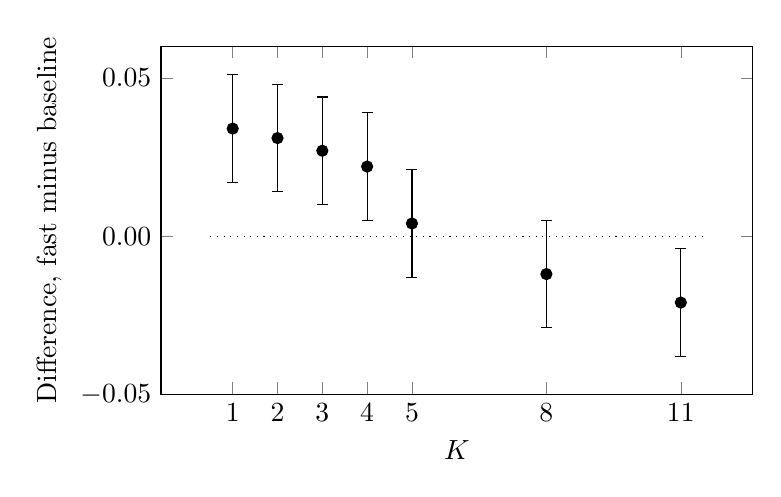
\begin{tikzpicture}
\begin{axis}[width=0.75\textwidth, height=6cm, xlabel={$K$}, ylabel={Difference, fast minus baseline}, xtick={1,2,3,4,5,8,11}, ymin=-0.05, ymax=0.06, scaled y ticks=false]
\addplot[mark=*, only marks, error bars/.cd, y dir=both, y explicit] coordinates {
(1,0.034) +- (0,0.017)
(2,0.031) +- (0,0.017)
(3,0.027) +- (0,0.017)
(4,0.022) +- (0,0.017)
(5,0.004) +- (0,0.017)
(8,-0.012) +- (0,0.017)
(11,-0.021) +- (0,0.017)
};
\addplot[dotted] coordinates {(0.5,0) (11.5,0)};
\end{axis}
\end{tikzpicture}
\caption{Effect of fast turnover on long-run performance, delegated structure. Points are differences in mean long-run performance between fast ($\tau = 0.10$) and baseline ($\tau = 0.02$) turnover; bars are 95 percent intervals (the difference plus or minus 1.96 standard errors). Standard deviation across runs is 0.06 in each condition, with 100 runs per condition.}
\label{fig:turnover}
\end{figure}

\subsection{A large-sample test}

Appendix C shows that the gap between the two structures narrows as $K$ rises from 5 to 7. To test whether delegation still holds an advantage in this range, we reran the comparison at $K = 6$ with 10,000 runs per condition, again using independently drawn landscapes for each condition and 250 periods per run. Table~\ref{tab:signif} reports the results. The advantage of delegation is significant at p < 0.001, confirming that delegation outperforms centralization at this level of interdependence.

\begin{table}[h]
\centering
\caption{Large-sample comparison, $K = 6$}
\label{tab:signif}
\begin{tabular}{lcc}
\toprule
 & Delegated & Centralized \\
\midrule
Long-run performance & 0.709*** & 0.705 \\
Runs per condition & 10,000 & 10,000 \\
\bottomrule
\end{tabular}

\smallskip
\footnotesize Note: *** delegated mean differs from centralized mean at p < 0.001, two-sided test of the difference in means across runs.
\end{table}

\section{Mechanism}

Why does delegation help? We attribute the advantage of delegation to filtering by middle managers. A unit manager sees only the unit's own performance and screens candidate changes against it. Changes that would help the whole organization but hurt the unit are filtered out, and changes that help the unit but hurt the whole are let through. This filtering keeps the delegated organization moving across the landscape after a centralized organization would have stopped, and it is this movement that lets delegated organizations reach better regions of a rugged landscape.

The filtering account fits the pattern of our results. Filtering matters most when many decisions are interdependent, because that is when a unit's partial view departs most from the view of the whole. It also explains why three units outperform two in Table~\ref{tab:main}: with more units, each manager's view is narrower and filtering is stronger. Middle managers, on this account, are not a cost of delegation but its source of value.

\section{Implications}

Our results carry a direct message for practice. Firms should delegate at least 40 percent of decisions when their operations are highly interdependent. Below that share, the filtering that unit managers provide is too weak to move the organization off inferior configurations.

The results also suggest a broader idea about organizations. When interdependence is low or moderate, the partial views of unit managers may be an asset rather than a liability, because partial evaluation keeps an organization searching. We offer this as a proposition for field studies of delegation: organizations facing tasks of low or moderate interdependence should, other things equal, benefit from dispersing decision rights. Testing this proposition requires measures of task interdependence and of the allocation of decision rights, both of which field research can supply.

\section{Extension: Teams of LLM Agents}

\subsection{Setup}

Recent advances in large language models make it possible to replace rule-based agents with agents that reason in natural language. We extend the delegated structure by replacing each unit manager with an LLM agent. Each agent is an instance of the open-weights model Llama 3.1 8B Instruct (model version Llama-3.1-8B-Instruct, weights accessed on 12 March 2026 and run locally), sampled at a temperature of 0.7 with a limit of 300 output tokens per response. All agents in all runs use the same model and the same prompt, printed in full in Appendix D.

Each period, each agent receives its unit's current decisions, the unit's current performance, and the performance of one candidate change, and replies with a proposal and a short justification addressed to the other unit managers. Each agent sees the last five messages from its team. We ran 20 runs of 50 periods each with two units, on landscapes drawn as in Section 3 with $K = 5$.

\subsection{Validation}

To validate the LLM agents, we read their exchanges. Three are typical:

\begin{quote}\small
Unit 1: ``Switching supplier routine 3 raises our unit score from 0.61 to 0.64. I propose we adopt it, though it may affect scheduling in Unit 2.''\\
Unit 2: ``Noted. Our scheduling score dropped slightly last period. I will hold my change this round so we can see the effect of yours.''
\end{quote}

\begin{quote}\small
Unit 2: ``The inspection change did not help. I am reverting it and will try the pricing tier instead.''
\end{quote}

\begin{quote}\small
Unit 1: ``We have not improved in four periods. I suggest we each try a change we rejected earlier.''\\
Unit 2: ``Agreed. I will revisit the batch-size rule.''
\end{quote}

In these and other exchanges, the agents behaved in realistic ways: they explained their choices, responded to one another, and changed course when a change failed. LLM teams reached a mean long-run performance of 0.698 over the 50 periods.

\subsection{Emergent coordination}

We also placed the agents in a naming game. In each of 20 runs, ten agents were paired at random each round and asked to agree on a name for an abstract symbol, with a reward when both partners gave the same name. Within 30 rounds, the agents in 18 of the 20 runs spontaneously converge on a shared naming convention, and they keep it for the rest of the run. We read this as emergent coordination: without any central instruction, teams of LLM agents develop shared conventions that let them act together.

\section{Conclusion}

We built an NK model of delegated and centralized search and found that delegation outperforms centralization in complex environments. The result points to the value of partial views inside organizations and to the role of middle managers in sustaining search. Future work can extend the model to richer structures, including hierarchies with several levels and units that share decisions.

\section*{Code and Data Statement}

The simulation was written in Python. Code is available from the authors upon reasonable request. The model uses no external data.

\begin{thebibliography}{9}

\bibitem[Baumann et al.(2019)]{baumann2019}
Baumann, O., Schmidt, J., and Stieglitz, N. 2019. Effective search in rugged performance landscapes: A review and outlook. \textit{Journal of Management} 45(1): 285--318.

\bibitem[Csaszar(2018)]{csaszar2018}
Csaszar, F. A. 2018. A note on how NK landscapes work. \textit{Journal of Organization Design} 7: article 15.

\bibitem[Davis et al.(2007)]{davis2007}
Davis, J. P., Eisenhardt, K. M., and Bingham, C. B. 2007. Developing theory through simulation methods. \textit{Academy of Management Review} 32(2): 480--499.

\bibitem[Grimm et al.(2020)]{grimm2020}
Grimm, V., Railsback, S. F., Vincenot, C. E., Berger, U., Gallagher, C., DeAngelis, D. L., Edmonds, B., Ge, J., et al. 2020. The ODD protocol for describing agent-based and other simulation models: A second update to improve clarity, replication, and structural realism. \textit{Journal of Artificial Societies and Social Simulation} 23(2): 7.

\bibitem[Levinthal(1997)]{levinthal1997}
Levinthal, D. A. 1997. Adaptation on rugged landscapes. \textit{Management Science} 43(7): 934--950.

\end{thebibliography}

\clearpage
\appendix
\section*{Appendix A. Model Assumptions}
\addcontentsline{toc}{section}{Appendix A}
\renewcommand{\thetable}{A\arabic{table}}
\renewcommand{\thefigure}{A\arabic{figure}}
\setcounter{table}{0}
\setcounter{figure}{0}

The model rests on the following assumptions, which hold in every experiment unless stated otherwise.

\begin{enumerate}
\item[A.1] Decisions are binary, and the organization makes all $N = 12$ decisions in every period.
\item[A.2] Managers observe the value of their performance measure exactly, without noise, for the current configuration and for the candidate change they evaluate.
\item[A.3] Units do not communicate in the rule-based model. A unit manager observes only the decisions under the unit's control and the unit's own performance.
\item[A.4] Each delegated unit may change up to two decisions per period, each by a one-bit move evaluated as in Section 3.2, while the centralized structure changes at most one decision per period.
\item[A.5] A manager who arrives through turnover inherits the unit's current decisions and has no memory of earlier periods.
\item[A.6] The landscape is fixed within a run; there is no environmental change.
\end{enumerate}

Table~\ref{tab:units} shows how decisions are assigned to units in the two delegated structures of Table~\ref{tab:main}. Table~\ref{tab:sd} reports the standard deviation of long-run performance across runs for each condition in Table~\ref{tab:main}, and Table~\ref{tab:sdlarge} does the same for the large-sample comparison of Section 4.3.

\begin{table}[h]
\centering
\caption{Assignment of decisions to units}
\label{tab:units}
\begin{tabular}{lll}
\toprule
Structure & Unit & Decisions \\
\midrule
Two units & Unit 1 & $d_1$--$d_6$ \\
 & Unit 2 & $d_7$--$d_{12}$ \\
Three units & Unit 1 & $d_1$--$d_4$ \\
 & Unit 2 & $d_5$--$d_8$ \\
 & Unit 3 & $d_9$--$d_{12}$ \\
\bottomrule
\end{tabular}
\end{table}

\begin{table}[h]
\centering
\caption{Dispersion of long-run performance across runs, $K = 5$}
\label{tab:sd}
\begin{tabular}{clcc}
\toprule
Row of Table~\ref{tab:main} & Condition & SD across runs & Runs \\
\midrule
1 & Delegated, two units & 0.06 & 100 \\
1 & Centralized & 0.06 & 100 \\
2 & Delegated, three units & 0.06 & 100 \\
2 & Centralized & 0.06 & 100 \\
\bottomrule
\end{tabular}

\smallskip
\footnotesize Note: Each condition is run on independently drawn landscapes.
\end{table}

\begin{table}[h]
\centering
\caption{Dispersion of long-run performance across runs, large-sample comparison, $K = 6$}
\label{tab:sdlarge}
\begin{tabular}{lcc}
\toprule
Condition & SD across runs & Runs \\
\midrule
Delegated, two units & 0.05 & 10,000 \\
Centralized & 0.05 & 10,000 \\
\bottomrule
\end{tabular}

\smallskip
\footnotesize Note: Each condition is run on independently drawn landscapes.
\end{table}

\clearpage
\section*{Appendix B. Sensitivity Analysis}
\addcontentsline{toc}{section}{Appendix B}

We vary each parameter in turn, holding the others at baseline. Figure~\ref{fig:units} varies the number of units under delegation from one to six at $K = 5$ and $\tau = 0.02$. Figure~\ref{fig:tau} varies the turnover rate from 0 to 0.20 at $K = 5$ with two units. In both sweeps, delegated organizations with two or more units match or exceed the centralized benchmark, and we conclude that the headline result is robust.

\begin{figure}[h]
\centering
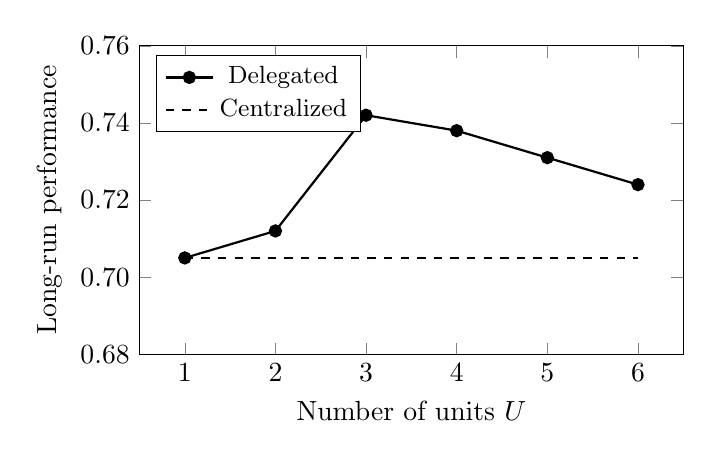
\begin{tikzpicture}
\begin{axis}[width=0.7\textwidth, height=5.5cm, xlabel={Number of units $U$}, ylabel={Long-run performance}, ymin=0.68, ymax=0.76, xtick={1,2,3,4,5,6}, legend pos=north west, legend style={font=\small}]
\addplot[mark=*, thick] coordinates {(1,0.705) (2,0.712) (3,0.742) (4,0.738) (5,0.731) (6,0.724)};
\addlegendentry{Delegated}
\addplot[dashed, thick] coordinates {(1,0.705) (6,0.705)};
\addlegendentry{Centralized}
\end{axis}
\end{tikzpicture}
\caption{Long-run performance by number of units, $K = 5$, $\tau = 0.02$}
\label{fig:units}
\end{figure}

\begin{figure}[h]
\centering
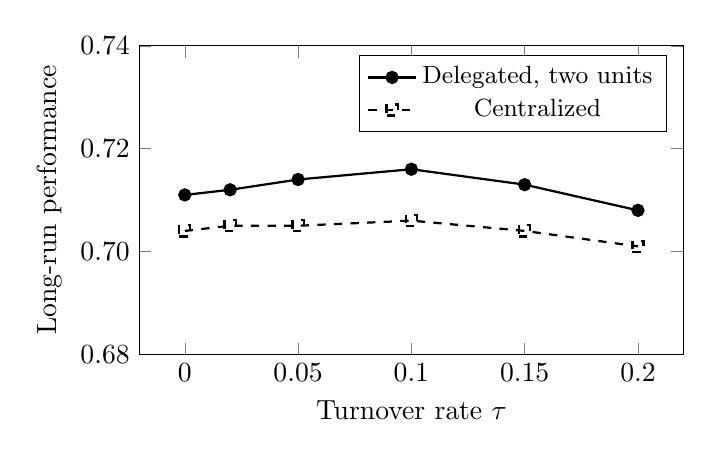
\begin{tikzpicture}
\begin{axis}[width=0.7\textwidth, height=5.5cm, xlabel={Turnover rate $\tau$}, ylabel={Long-run performance}, ymin=0.68, ymax=0.74, xtick={0,0.05,0.10,0.15,0.20}, scaled x ticks=false, xticklabel style={/pgf/number format/fixed, /pgf/number format/precision=2}, legend pos=north east, legend style={font=\small}]
\addplot[mark=*, thick] coordinates {(0,0.711) (0.02,0.712) (0.05,0.714) (0.10,0.716) (0.15,0.713) (0.20,0.708)};
\addlegendentry{Delegated, two units}
\addplot[mark=square, dashed, thick] coordinates {(0,0.704) (0.02,0.705) (0.05,0.705) (0.10,0.706) (0.15,0.704) (0.20,0.701)};
\addlegendentry{Centralized}
\end{axis}
\end{tikzpicture}
\caption{Long-run performance by turnover rate, $K = 5$, two units}
\label{fig:tau}
\end{figure}

\clearpage
\section*{Appendix C. Results Across Levels of Interdependence}
\addcontentsline{toc}{section}{Appendix C}

The main text reports results at $K = 5$. Figure~\ref{fig:k} reports long-run performance under both structures for every value of $K$ from 0 to 11, with two units, $\tau = 0.02$, and 100 runs per condition. At $K = 0$ both structures reach the same long-run performance. Delegation performs better from $K = 1$ through moderate levels of interdependence, and the gap narrows between $K = 5$ and $K = 7$. For K of 8 or more, centralized search performs better, as panel (c) shows.

\begin{figure}[h]
\centering
\begin{subfigure}{0.32\textwidth}
\centering
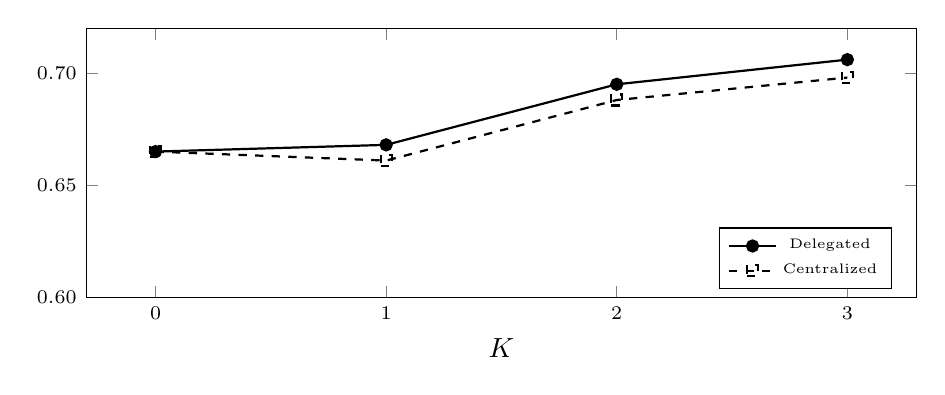
\begin{tikzpicture}
\begin{axis}[width=\textwidth, height=5cm, xlabel={$K$}, ymin=0.60, ymax=0.72, xtick={0,1,2,3}, tick label style={font=\scriptsize}, legend style={font=\tiny, at={(0.97,0.03)}, anchor=south east}]
\addplot[mark=*, thick] coordinates {(0,0.665) (1,0.668) (2,0.695) (3,0.706)};
\addlegendentry{Delegated}
\addplot[mark=square, dashed, thick] coordinates {(0,0.665) (1,0.661) (2,0.688) (3,0.698)};
\addlegendentry{Centralized}
\end{axis}
\end{tikzpicture}
\caption{$K$ from 0 to 3}
\end{subfigure}
\hfill
\begin{subfigure}{0.32\textwidth}
\centering
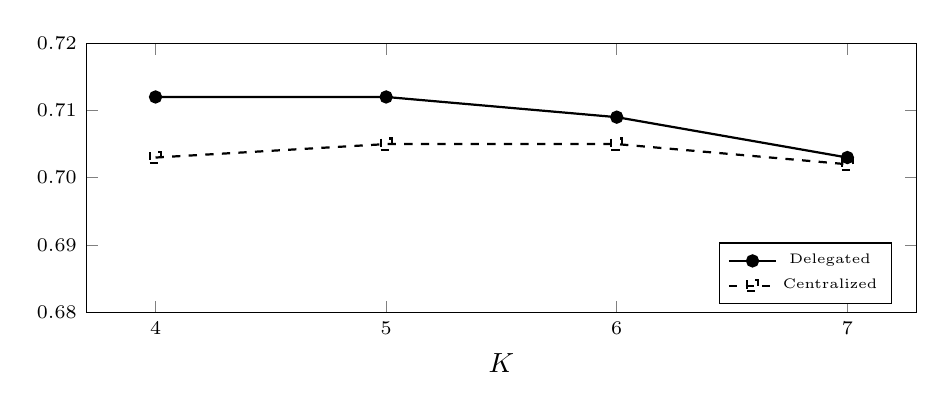
\begin{tikzpicture}
\begin{axis}[width=\textwidth, height=5cm, xlabel={$K$}, ymin=0.68, ymax=0.72, xtick={4,5,6,7}, tick label style={font=\scriptsize}, legend style={font=\tiny, at={(0.97,0.03)}, anchor=south east}]
\addplot[mark=*, thick] coordinates {(4,0.712) (5,0.712) (6,0.709) (7,0.703)};
\addlegendentry{Delegated}
\addplot[mark=square, dashed, thick] coordinates {(4,0.703) (5,0.705) (6,0.705) (7,0.702)};
\addlegendentry{Centralized}
\end{axis}
\end{tikzpicture}
\caption{$K$ from 4 to 7}
\end{subfigure}
\hfill
\begin{subfigure}{0.32\textwidth}
\centering
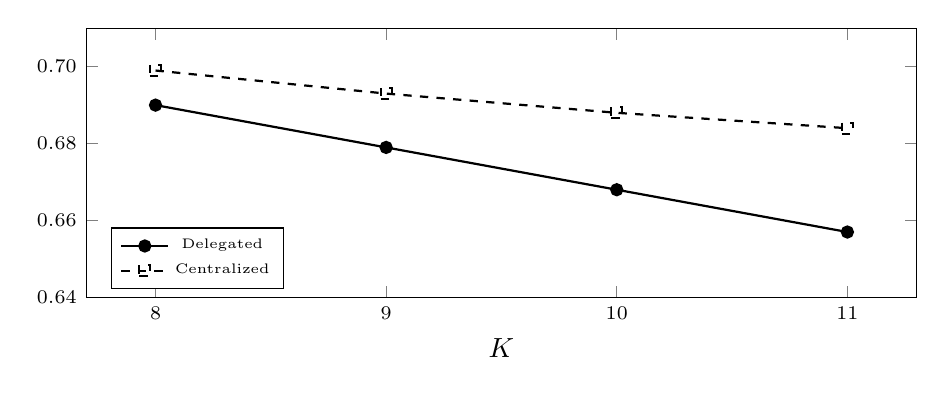
\begin{tikzpicture}
\begin{axis}[width=\textwidth, height=5cm, xlabel={$K$}, ymin=0.64, ymax=0.71, xtick={8,9,10,11}, tick label style={font=\scriptsize}, legend style={font=\tiny, at={(0.03,0.03)}, anchor=south west}]
\addplot[mark=*, thick] coordinates {(8,0.690) (9,0.679) (10,0.668) (11,0.657)};
\addlegendentry{Delegated}
\addplot[mark=square, dashed, thick] coordinates {(8,0.699) (9,0.693) (10,0.688) (11,0.684)};
\addlegendentry{Centralized}
\end{axis}
\end{tikzpicture}
\caption{$K$ from 8 to 11}
\end{subfigure}
\caption{Long-run performance by level of interdependence, two units, $\tau = 0.02$}
\label{fig:k}
\end{figure}

\clearpage
\section*{Appendix D. Prompts for the LLM Extension}
\addcontentsline{toc}{section}{Appendix D}

Every agent received the following system prompt, with the bracketed fields filled in for its unit.

\begin{quote}\small\ttfamily
You are the manager of [UNIT NAME] at a manufacturing firm. You control the following operational decisions: [LIST OF DECISIONS AND CURRENT SETTINGS]. Each period you may propose to change one of your decisions. Your goal is to raise your unit's performance score. You will be told your unit's current score and the score your unit would have if the candidate change were adopted. Write one short message to the other unit managers stating whether you adopt the change and why. Keep your message under 60 words.
\end{quote}

Each period, the agent then received the following user message.

\begin{quote}\small\ttfamily
Period [T]. Your unit's current score is [CURRENT SCORE]. Candidate change: set [DECISION] to [VALUE]. Score if adopted: [CANDIDATE SCORE]. Recent messages from your team: [LAST FIVE MESSAGES]. State whether you adopt the change, then write your message.
\end{quote}

In the naming game of Section 7.3, each agent received the following prompt each round.

\begin{quote}\small\ttfamily
You are playing a game with a partner. You both see the symbol shown below. Give it a one-word name. If you and your partner give the same name, you both earn a point. Names you and your partners used in earlier rounds: [HISTORY]. Symbol: [SYMBOL]. Reply with the name only.
\end{quote}

\end{document}
